\documentclass{article}
\usepackage{array}
\newcolumntype{L}{>{\centering\arraybackslash}m{4cm}}
\usepackage[czech]{babel}
\usepackage[utf8]{inputenc}
\usepackage[unicode]{hyperref}
\usepackage{graphicx}
\usepackage{textcomp}
\usepackage[T1]{fontenc}
\usepackage[left=2cm, text={17cm, 24cm}, top=2cm]{geometry}
\usepackage[table,xcdraw]{xcolor}
\usepackage{caption}
\usepackage{color}
\usepackage{hyperref}
\hypersetup{
    colorlinks=true, % make the links colored
    linkcolor=blue, % color TOC links in blue
    urlcolor=red, % color URLs in red
    linktoc=all % 'all' will create links for everything in the TOC
}

\begin{document}

%%%%%%%%%%%%%%%%%TITULKA%%%%%%%%%%%%%%%%%% 

	\begin{titlepage}
		\begin{center}
			\textsc{\Huge Vysoké Učení Technické v Brně} \\[0.7cm]
			{\Huge Fakulta informačních technologií}
			\center
\includegraphics[width=0.5\linewidth]{./logo.png}\\[5cm]

            \textbf{{\Huge Databázové systémy 2020}}\\[0.5cm]

			\textbf{{\huge Dokumentácia k projektu}}\\[0.4cm]
			\LARGE{Svet mágie}\\
			
		\end{center}
		\vfill

		\begin{flushleft}
			\begin{Large}
				\textbf{Marek Žiška}\hspace{44px}\textbf{(xziska03)}\\[0.25cm]
				\textbf{Martin Osvald}\hspace{30px}\textbf{(xosval03)}
			\hfill
			Brno, 30.04.2020
			\end{Large}
		\end{flushleft}

	\end{titlepage}
    \tableofcontents
    \newpage
    \section{Úvod a zadanie}
    \subsection{Úvod}
    \Large{Tento dokument popisuje návrh a implementáciu databáze zo zadania z predmetu Úvod do softwarového inžinierstva, svet mágie.}
    \subsection{Zadanie}
    \Large{Kouzelnický svět vytváří informační systém pro evidence kouzel a kouzelníků. Magie v kouzelnickém světě je členěna podle elementů (např. voda, oheň, vzduch,.), které mají různé specializace (obrana, útok, podpora,.) a různé, ale pevně dané, barvy magie (např. ohnivá magie je pomerančově oranžová). Každé kouzlo má pak jeden hlavní element a může mít několik vedlejších elementů (např. voda a led), přičemž každý kouzelník má positivní synergii s určitými elementy. U kouzelníků rovněž evidujeme velikost many, jeho dosaženou úroveň v kouzlení (předpokládáme .klasickou stupnici. E, D, C, B, A, S, SS,.). U jednotlivých kouzel pak jejich úroveň složitosti seslání, typ (útočné, obranné) a sílu. Kouzla všaknemohou být samovolně sesílána, pouze s využitím kouzelnických knih, tzv. grimoárů. Grimoáry v sobě seskupují více připravených kouzel a uchováváme veškerou historii jejich vlastnictví. Grimoáry mohou obsahovat kouzla různých elementů, nicméně jeden z elementů je pro ně primární, přičemž může obsahovat přibližně 10-15 kouzel. S postupem času však grimoáry ztrácejí nabitou magii (přibližně po měsíci ztratí veškerou magii) a je nutno je znovu dobít, ale pouze na dedikovaných místech, kde prosakuje magie (míra prosakování magie daného místa je evidována) určitých typů element (předpokládejte, že na daném místě prosakuje právě jeden typ). Toto nabití však nemusí být provedeno vlastníkem, ale I jiným kouzelníkem. V případě blížícího se vypršení magie grimoáru, systém zašle upozornění vlastníkovi. Alternativním způsobem sesílání magie je pak s využitím svítku, který obsahuje právě jedno kouzlo a po jeho použití se rozpadne.}              
    \newpage
    
    \section{Návrh}
    \subsection{Generalizácia/špecializácia}
    \Large{Generalizáciu sme v zadaní s predmetu IUS nenašli tak sme si ju pridali. Pridali sme dve generalizácie, jednu pre tabuľku \textit{Kouzlo}, kde generalizácia bola kliatba o ktorej sme navyše evidovali trvanie kliatby.}\\
    \Large{Druhú generalizáciu sme vytvorili pre tabuľku \textit{Magická bytost}, boli to \textit{Kouzelnik} a \textit{Elf}}
    \subsection{Er diagram}
    \begin{center}\\[1cm]
    \hspace*{-2cm} 
    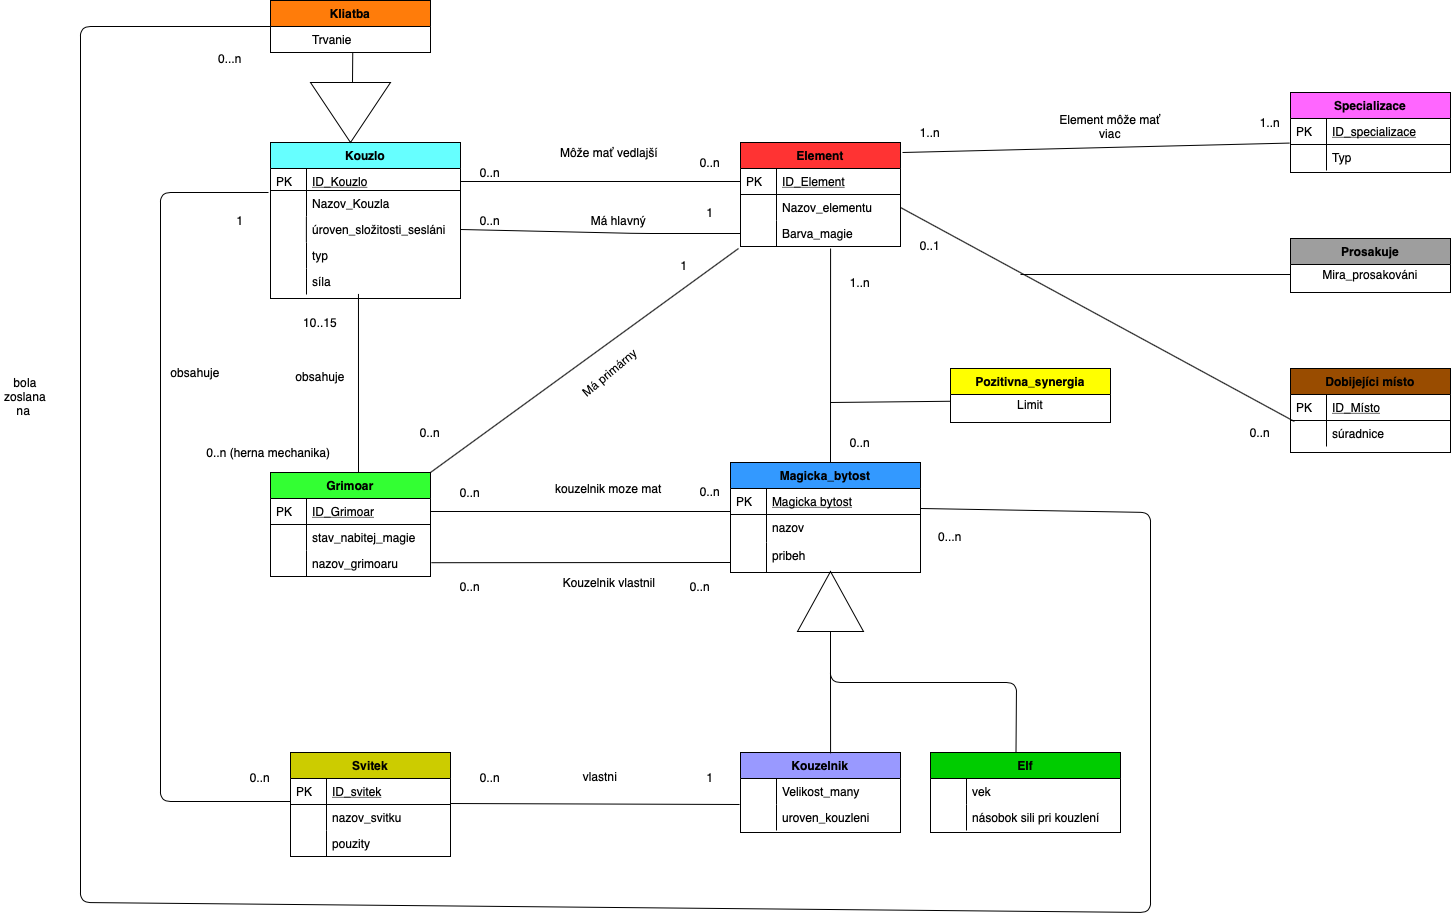
\includegraphics[width=1.25\linewidth]{./erdiagram.png}
    \end{center}
    \newpage
    \subsection{Use case diagram}
    \begin{center}[4cm]
    \hspace*{-2cm} 
    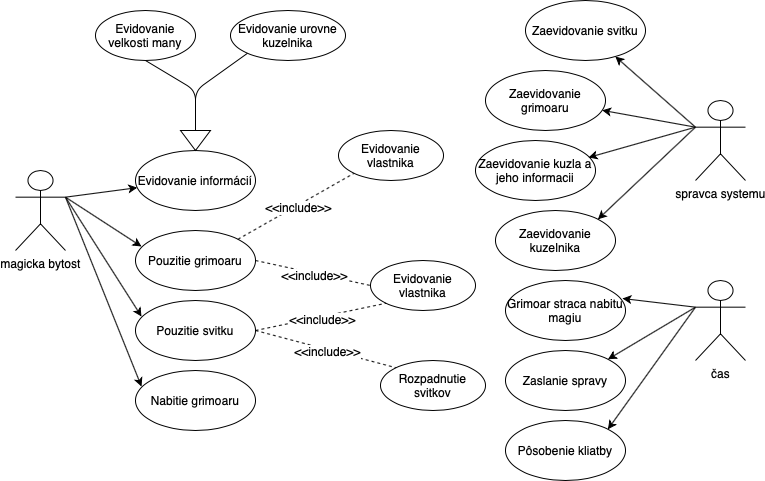
\includegraphics[width=1.25\linewidth]{./usecase.png}
    \end{center}
    
    \newpage
    \section{Vytvorenie tabuliek}
    \subsection{Zoznam tabuliek}
    \Large{Zoznam finálne vytvorených tabuliek predstavujúce jednotlivé entity, a niektoré many to many vzťahy.}
    \begin{itemize}
	\item CHARGING\_PLACE
	\item SECONDARY\_ELEMENTS
	\item SPELL
	\item ELEMENT\_SPECIALIZATION
	\item SPECIALIZATION
	\item CURSED\_BEING
	\item POSITIVE\_SYNERGY
	\item SCROLL
	\item MAGICAL\_BEING
	\item MAGICAL\_BEING\_CAN\_HAVE
	\item MAGICAL\_BEING\_HAD
	\item GRIMOIRE
	\item GRIMOIRE\_CONTAINS\_SPELLS
	\item ELEMENT
    \end{itemize}
    \subsection{Naplnenie dátami}
    \Large{Tabuľku sme naplnili demo dátami pomocou internetového nástroja, plus sme niektoré dáta sme pridali ručne pre rozumnú demonštráciu funkčnosti našich skriptov.}\\[0.4cm]
    \subsection{Reprezentácia databázy}
    \center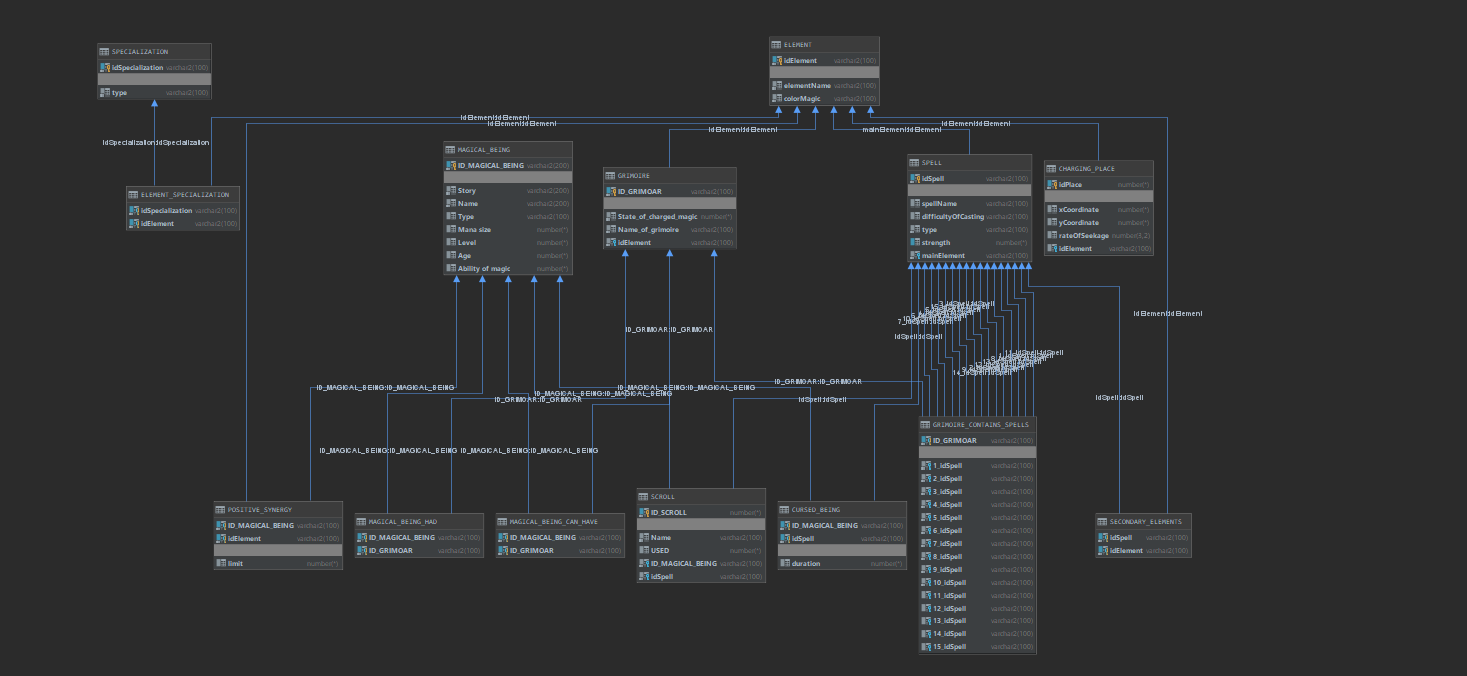
\includegraphics[width=1\linewidth]{./unknown.png}\\[5cm]
    \newpage
    \section{Select skripty}
    \Large{Vytvorili sme sedem skriptov, ktoré spĺňajú všekty požiadavky zo zadania.}\\
    \Large{Prvý skript dotazoval, ktorý kúzelníci vlastnili svitok. Tento a druhý skript pužívali spojenie dvoch tabuliek.}
    \begin{verbatim}
    Select scroll."Name" , magic_being."Name" From
    ( Select * From SCROLL ) scroll
    inner join
    ( Select * From MAGICAL_BEING) magic_being
    on scroll.ID_MAGICAL_BEING  = magic_being.ID_MAGICAL_BEING ;
    \end{verbatim}
    \Large{Druhý skript sa dotazoval na to aké kúzla majú hlavný element s farbou Indigo ?}
    \begin{verbatim}
    Select spells."spellName" , elements."elementName" from
    ( Select * from SPELL ) spells
    inner join
    ( Select * From ELEMENT where "colorMagic" = 'Indigo' ) elements
    on spells."mainElement" = elements."idElement";
    \end{verbatim}
    \Large{Tretí skript hľadal element ktorý má pozitívnu synergiu s nejakou magickou bytosťou a súčasne má špecializáciu s typom "turpis". Pri realizácií tohoto skriptu sme použili spojenie troch tabuliek}\\
    \Large{Štvrtý skript hľadal koľko kúziel majú jednotlivé elementy s farbou magie 'Violet'. Štvrtý a piaty skript využívali agregačnú funkciu s group by.}\\
    \Large{Piaty skript hľadal koľko kuziel ma silu väčšiu ako 50.}\\
    \Large{Šiesty skript hľadal či existuju kuzelníci ktorí maju pozitivnu synergiu s elementom vacsiu ako 50 tak vypis bytosti s
    pozitivnou synergiou vacsou ako 50. Tento skript využíval predikát EXISTS}\\
    \newpage
    \section{Posledná časť projektu}
    \subsection{Triggery}
    \Large{Naimplementovali sme dva triggery.}\\[0.2cm]
    \Large{Prvý trigger \textit{onInsertElement} má za úlohu autoinkrementovať primárny kľúč tabuľky \textit{CHARGING\_PLACE}, ktorá predstavovala nabíjacie miesto pre element. Teda pri každom vložení nových hodnôt do tabuľky sa primárny kľúč zvýši o jedna. Trigger bol naimplementovaný pomocou sekvencie.}\\
    \begin{verbatim}
    DROP SEQUENCE SEQ;
    CREATE SEQUENCE SEQ START WITH 1 INCREMENT BY 1 NOCYCLE;
    
    CREATE OR REPLACE TRIGGER onInsertElement BEFORE
        INSERT ON CHARGING_PLACE
        FOR EACH ROW
    BEGIN
        SELECT SEQ.NEXTVAL INTO :new."idPlace"
        FROM DUAL;
    END;
    \end{verbatim}
    \Large{Druhý trigger sa stará o situáciu keď sa vytvára nový Grimoár tak daný admin ešte nevie aký hlavný kúzelný element bude mať daný grimoár. Toto za neho môže vyriešiť trigger ktorý dá defaultne vybraný element.}
    \begin{verbatim}
    CREATE OR REPLACE TRIGGER GRIMOIRE_TRIGGER BEFORE
    INSERT ON GRIMOIRE
    FOR EACH ROW
    WHEN ( NEW."idElement" IS NULL  )
    BEGIN
       :NEW."idElement" := 'elem01918';
    END;
    \end{verbatim}
    \newpage
    
    
    \subsection{Procedúry}
    \Large{Naimplementovali sme dve procedúry.}\\[0.2cm]
    \Large{Úlohou prvej procedúry \textit{spell\_avg\_strength}je spočítanie priemernej sily pre špecifický typ kúzla z evidovaných záznamov kúziel. Argumentom procedúry je typ kúzla, pre ktorý chceme vedieť priemernú silu. Pri implementácií sme využili \textit{CURSOR}, vďaka ktorému v cykle prechádzame záznamy v tabuľke \textit{SPELL}. Keďže nie všetky kúzla dávajú poškodenie, niektoré nemusia mať žiadnu silu, teda majú hodnotu sily 0. Z dôvodu týchto záznamov odchytávame výnimku \textit{ZERO\_DIVIDE}. V prípade neúspešného vyhľadávania alebo iných neočakávaných chybách odchytávame aj výnimku \textit{OTHERS}.}\\[1cm]

    \Large{Druhá procedúra mala za úlohu zistiť koľko percent kúziel má hlavný element, ktorý bol špecifikovaný v argumente procedúry. Znova sme využili \textit{CURSOR} a výnimky ako pri prvej procedúre.}
    \newpage
    
    
    \subsection{Explain plan}
    \Large{Príkaz \textit{EXPLAIN PLAN} zobrazuje  postupnosť nasledujúcich príkazov  a taktiež azobrazuje cenu pre každú operáciu  CPU a aj čas vykonania.}
    \Large{}
    \begin{center}
        \begin{verbatim}
    SELECT "SPELL"."idSpell" id
    FROM "SPELL"
    WHERE "SPELL"."strength" > 50
    GROUP BY "SPELL"."idSpell";
        \end{verbatim}
    \end{center}
    \Large{Výstup \textit{EXPLAIN PLAN}}
    \begin{center}\includegraphics[width=1\linewidth]{./explainlapng.png}\\[1cm]
    \end{center}
    \Large{Optimalizovať tento Select môžeme pomocou CREATE INDEX. CREATE INDEX nám vytvorí index na základe hodnôť vo vybratých stĺpcoch.}
    \begin{verbatim}
    CREATE INDEX INDEX_SPELL ON SPELL ("idSpell", "strength");
    \end{verbatim}
    \Large{Po optimalizácií CREATE INDEX  môžeme vidieť v stĺpci COST \%CPU optimalizovanie 4 jednotky.}
    \newpage
    
    \subsection{Materializovaný pohľad}
    \Large{Účel materializovaného pohľadu je rýchli prístup pri opakovanom žiadaní na nejaký pohľad
    Náš materializovaný pohľad sa skladá z troch selectov. Vybrali sme tento select kvôli tomu že uživateľ má rád špecifickú farbu „Indigo” , tým pádom ma ku nemu opakovaní prístup.
    }
    \begin{verbatim}
    CREATE  MATERIALIZED VIEW SPELLS_WITH_ELEMENTS_td
    CACHE
    BUILD IMMEDIATE
    ENABLE QUERY REWRITE
    AS
    -- Ktoré kúzla má hlavný element farbu Indigo ? Vypiste názov kúzla 
    -- a názov elementu
    Select spells."spellName" , elements."elementName" from
        ( Select * from SPELL ) spells
        inner join
        ( Select * From ELEMENT where "colorMagic" = 'Indigo' ) elements
    on spells."mainElement" = elements."idElement";
    \end{verbatim}
    \Large{Práva ku tejto tabulke udávame pomocou príkazu GRANT ALL ON SPELLS}
    \begin{verbatim}
    GRANT ALL ON SPELLS_WITH_ELEMENTS_td TO xosval03;
    \end{verbatim}
\end{document}